\chapter{Installation of a private cloud}
\label{chap:cloud}
\emph{In addition to network attacks against stand-alone network computers, some attacks against private clouds will be performed. In this chapter, the installation of a cloud environment using Windows Server 2012 R2 will be covered in detail.}

\section{Installation of Microsoft System Center 2012 R2 Virtual Machine Manager}

\subsection{Installation requirements}

Before installing System Center 2012 R2 VMM, some hardware - and software requirements must be met.

\paragraph{Hardware requirements (up to managing 150 hosts)}
\begin{table}[h]
\begin{tabular}{|l|l|}
\hline
Processor                                                                   & Dual-core of 2,8 GHz \\ \hline
RAM                                                                         & 4 GB                 \\ \hline
Hard disk space without a local VMM database                                & 40 GB                \\ \hline
Hard disk space with a local VMM database  & 150 GB               \\ \hline
\end{tabular}
\end{table}
$\;$ \\
When managing more than 150 hosts, it is recommended to use a dedicated computer for MSSQL Server. That is, to store the VMM database on a dedicated computer.
\paragraph{Software requirements}
\begin{itemize}
\item Microsoft .NET Framework 4.5 or higher
\item Windows Deployment and installation kit for Windows 8.1
\item Windows Server 2012 R2
\item Microsoft SQL Server 2012 (with or without SP1 and SP2)
\end{itemize}
\paragraph{Other requirements}
\begin{itemize}
\item The server where the VMM will be installed, must be a member of an Active Directory domain.
\item The server name cannot exceed 15 characters
\end{itemize}
\subsection{Generatl installation overview}
\ldots
\subsection{Pre-installation configuration}
Prior to installing VMM, some settings will be configured such as a static IP address and joining the server to an AD domain. The complete installation has been performed on a freshly installed Windows Server 2012 R2 as VM on a Windows Server 2012 R2 running Hyper-V. Make sure you are logged in as a Domain Admin.

In order to be able to join the server to a domain, a static IP must be set. Make sure the DNS servers point to the DNS servers of the AD domain.
$\;$ \\ \\
\noindent\begin{minipage}{\textwidth}
    \centering
    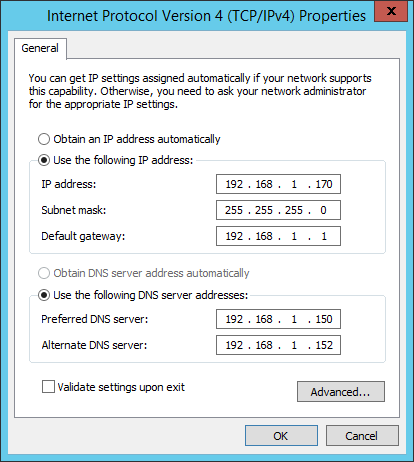
\includegraphics{Screenshots/vmmtest_IP.png}
 \captionof{figure}{configuring static IP settings.}
\end{minipage}
$\;$ \\ \\
After this, the server can be joined to the AD domain.
$\;$ \\ \\
\noindent\begin{minipage}{\textwidth}
    \centering
    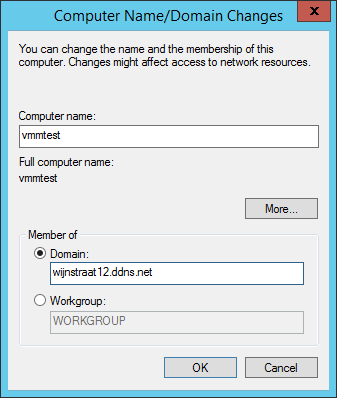
\includegraphics{Screenshots/vmmtest_Domain.png}
 \captionof{figure}{Setting an appropriate server name and joining the server to the AD domain.}
\end{minipage}
$\;$ \\ \\
\noindent\begin{minipage}{\textwidth}
    \centering
    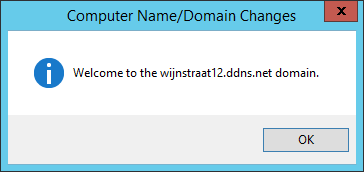
\includegraphics{Screenshots/vmmtest_Domain_2.png}
 \captionof{figure}{Confirmation of successfully joining the AD domain.}
\end{minipage}
$\;$ \\ \\
Next, the server has to be rebooted and the overview screen of the local server must be something as the figure below.
$\;$ \\ \\
\noindent\begin{minipage}{\textwidth}
    \centering
    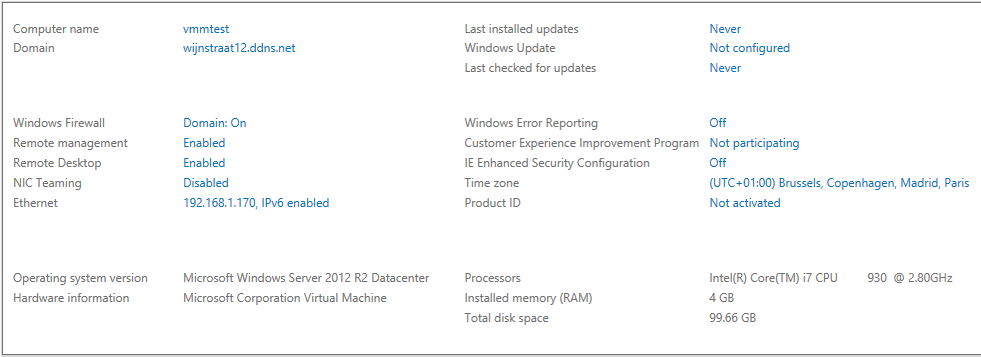
\includegraphics[width=\textwidth]{Screenshots/vmmtest_Overview.png}
 \captionof{figure}{The overview screen of the local server with a proper server name set, the server being joined to the domain, the firewall and remote desktop both being enabled. Also, a static IP has been set and the IE Enhanced Security Configuration has been disabled. Now we are ready to install Microsoft SQL Server 2012 SP2.}
\end{minipage}
$\;$ \\ 

\subsection{Installation of MSSQL Server 2012 SP2}

In this tutorial, SQL Server will be installed on the same server as the Virtual Machine Manager will be installed on. Before installing SQL Server 2012, the \texttt{netfx3} package will have to be installed, otherwise the installation process will fail. This is achieve by executing following command in PowerShell: \\
\texttt{dism /online /enable-feature /featurename:netfx3 /all /source:d:$\backslash$sources$\backslash$sxs} \\
Before executing this command, make sure that the installation media (that is, the .ISO image of WS2012R2) is inserted.
$\;$ \\ \\
\noindent\begin{minipage}{\textwidth}
    \centering
    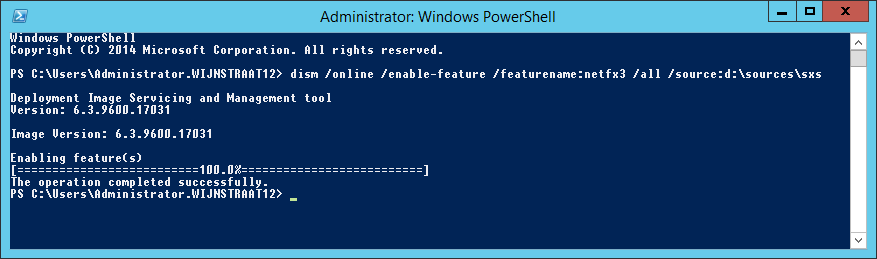
\includegraphics[width=\textwidth]{Screenshots/vmmtest_SQL_2.png}
 \captionof{figure}{\texttt{netfx3} has been installed successfully.}
\end{minipage}
$\;$ \\ \\
Now, the actual installation of SQL Server can begin. When mounting the SQL Server .ISO image and trying to run setup.exe, I expected some error messages. However, when first extracting the .ISO file with WinRAR and then executing setup.exe, everything went fine. 
$\;$ \\ \\
\noindent\begin{minipage}{\textwidth}
    \centering
     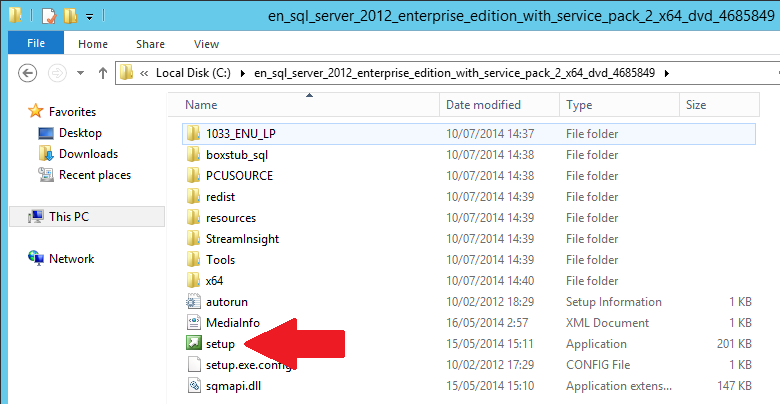
\includegraphics[width=\textwidth]{Screenshots/vmmtest_SQL_1.png}
 \captionof{figure}{Extract the image using WinRAR and run setup.exe.}
\end{minipage}
$\;$ \\ \\
\noindent\begin{minipage}{\textwidth}
    \centering
     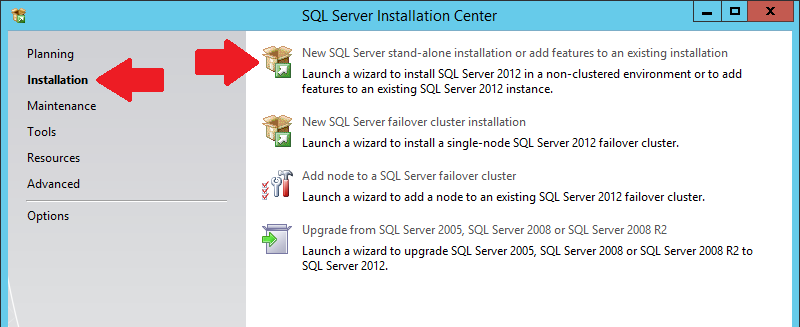
\includegraphics[width=\textwidth]{Screenshots/vmmtest_SQL_3.png}
 \captionof{figure}{In the left pane, select ``Installation'' and subsequently in the right pane, select ``New SQL Server stand-alone configuration''.}
\end{minipage}
$\;$ \\ \\
The installation will begin and the prerequisites will be checked. When every prerequisite is fulfilled, all marks will be green. Next, enter the product key or choose the evaluation version. After this, the license terms will have to be accepted and the installation will check for product updates.

When everything has been passed successfully, one should be seeing the following figure.
$\;$ \\ \\
\noindent\begin{minipage}{\textwidth}
    \centering
    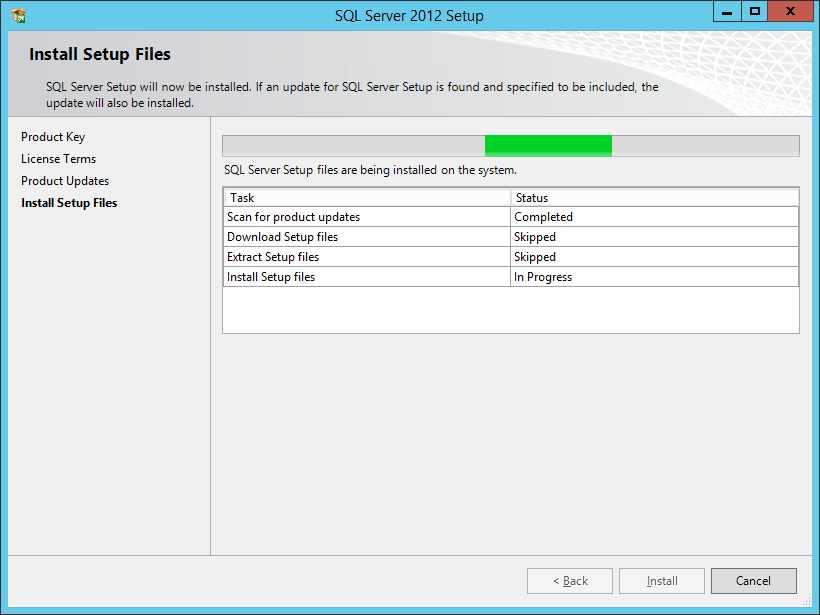
\includegraphics[width=\textwidth]{Screenshots/vmmtest_SQL_4.png}
 \captionof{figure}{Setup files are being installed.}
\end{minipage}
$\;$ \\ \\
Some additional prerequisites are checked. When everything is passed, setup can be continued. 
$\;$ \\ \\
\noindent\begin{minipage}{\textwidth}
    \centering
    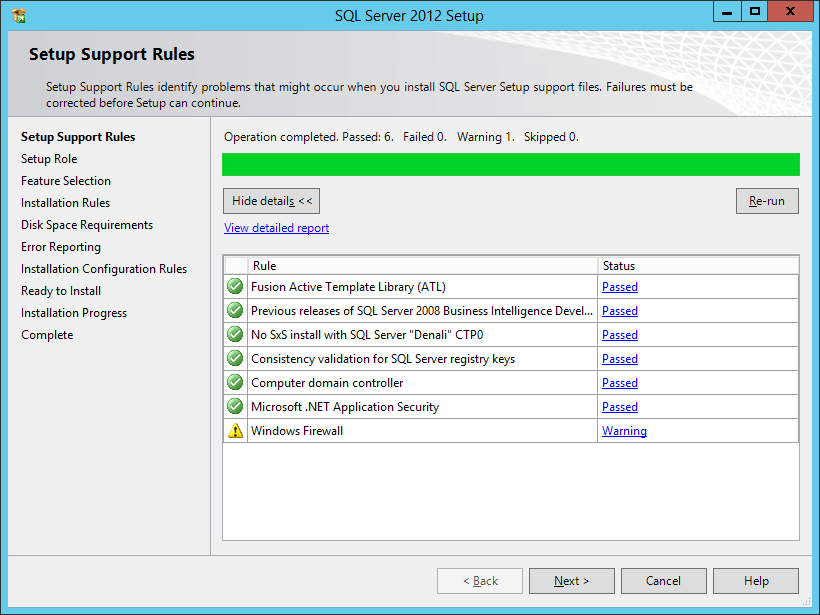
\includegraphics[width=\textwidth]{Screenshots/vmmtest_SQL_5.png}
 \captionof{figure}{Checking additional prerequisites.}
\end{minipage}
$\;$ \\ \\
On the feature selecting screen, make sure the following features are checked:
\begin{itemize}
\item Database Engine Services
\item Management Tools - Basic
\item Management Tools - Advanced
\item SQL Client connectivity SDK
\end{itemize}
$\;$ \\ \\
\noindent\begin{minipage}{\textwidth}
    \centering
    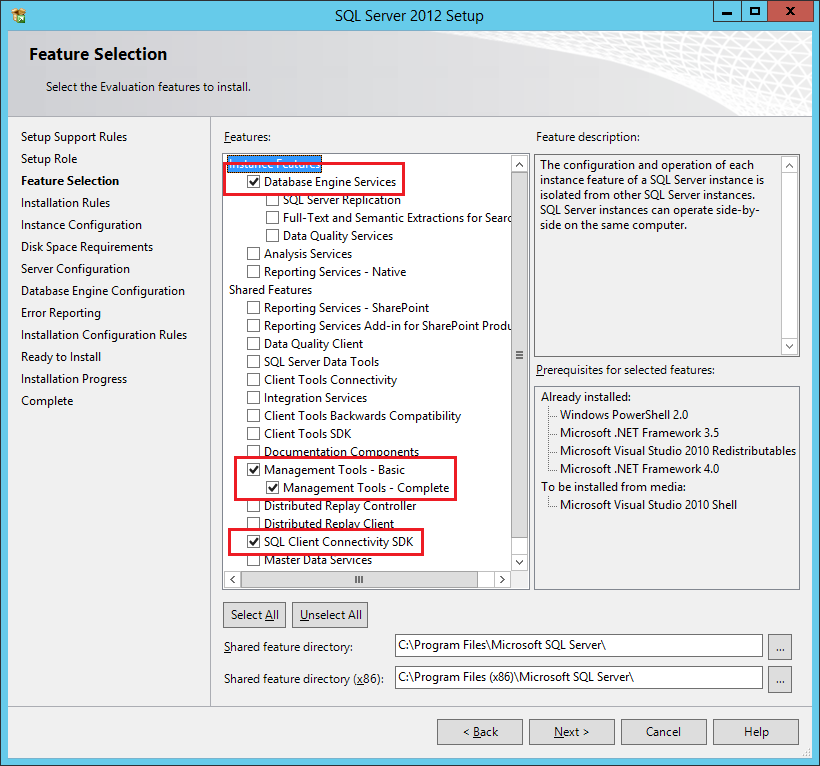
\includegraphics[width=\textwidth]{Screenshots/vmmtest_SQL_6.png}
 \captionof{figure}{Selection of the features.}
\end{minipage}
$\;$ \\ \\
On the next screen, choose ``Windows Authentication Mode'' and specify the administrators. In this case, both Domain Admins as well as Local Admins have been chosen.
$\;$ \\ \\
\noindent\begin{minipage}{\textwidth}
    \centering
    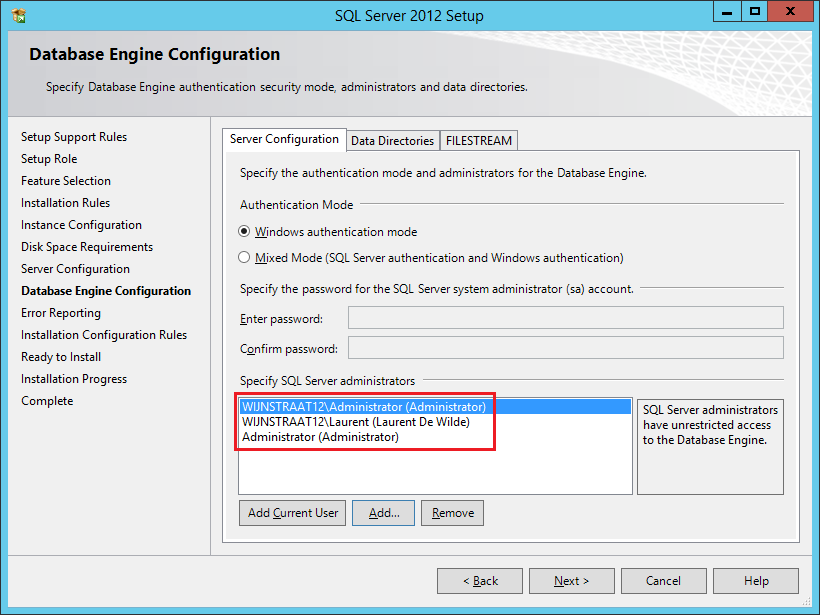
\includegraphics[width=\textwidth]{Screenshots/vmmtest_SQL_7.png}
 \captionof{figure}{Windows Authentication Mode is chosen and the SQL administrators are added.}
\end{minipage}
$\;$ \\ \\
\noindent\begin{minipage}{\textwidth}
    \centering
    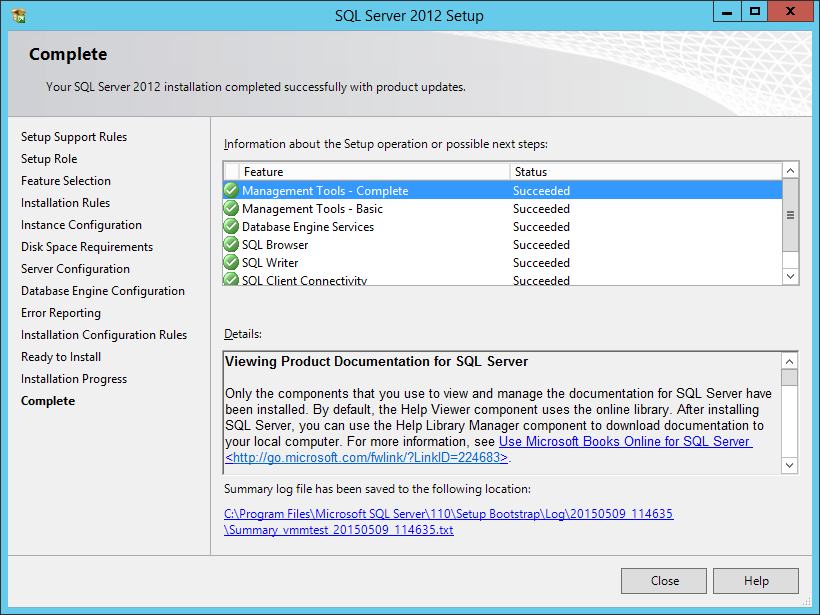
\includegraphics[width=\textwidth]{Screenshots/vmmtest_SQL_8.png}
 \captionof{figure}{Setup has completed successfully.}
\end{minipage}
$\;$ \\

\subsection{Configuring Distributed Key Management in Active Directory}
Distributed key management is used when a VMM cluster is used. The database of VMM is encrypted because it contains sensitive data. Consider the situation where two servers are used to form a clustered VMM environment. If the decryption keys are stored locally on server 1 and this particular server goes offline, there is no way to access the decryption keys anymore. This is why the keys are stored in a special container in Active Directory. This way, anytime access to the decryption keys is guaranteed. \\
In combination with DKM, a service account needs to be as well. This account is used to, for example, share .ISO images in the shared libraries of VMM.

Let us configure Distributed Key Management (DKM) and the service account. \\ \\
To do so, a new OU named ``ServiceAccounts'' is made under the root domain in the ``Active Directory Users and Groups'' snap-in. In this newly created OU, a (domain)user ``VMMService'' is made. This user serves as the service account for VMM.

Make sure that the password never expires.
$\;$ \\ \\
\noindent\begin{minipage}{\textwidth}
    \centering
    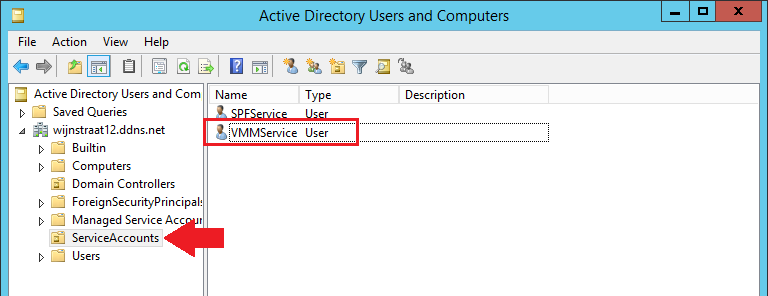
\includegraphics[width=\textwidth]{Screenshots/vmmtest_AD_1.png}
 \captionof{figure}{Making the service account for DKM.}
\end{minipage}
$\;$ \\ \\
\noindent\begin{minipage}{\textwidth}
    \centering
    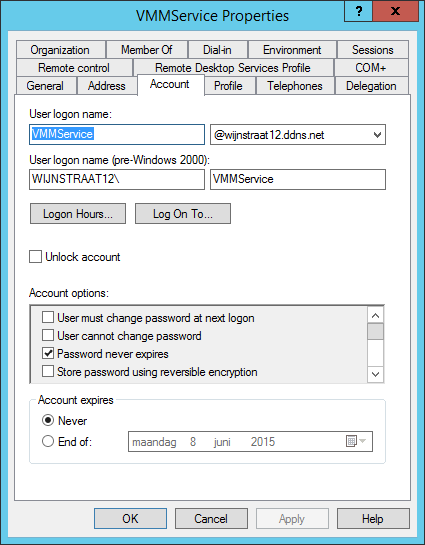
\includegraphics{Screenshots/vmmtest_AD_2.png}
 \captionof{figure}{The properties of the service account.}
\end{minipage}
$\;$ \\ \\
Now, the actual container for the keys can be made in Active Directory. To do so, open ``ADSI Edit'' from the local server overview of the server manager: \texttt{Server Manager $\rightarrow$ Local Server $\rightarrow$ Tools $\rightarrow$ ADSI Edit}. \\
Accept the default naming context (click \texttt{OK}) and expand the \texttt{Default naming context} node. Right click on the root OU and choose \texttt{New $\rightarrow$ Object}. \\
Select \texttt{container} and name it for example ``VMMDKM''. Click \texttt{Finish}. 
$\;$ \\ \\
\noindent\begin{minipage}{\textwidth}
    \centering
    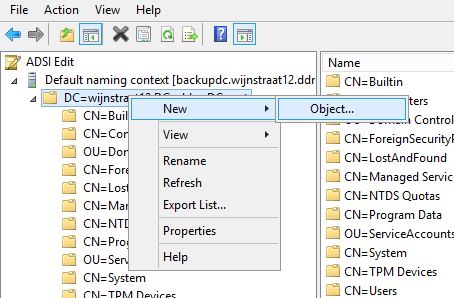
\includegraphics{Screenshots/vmmtest_AD_3.png}
 \captionof{figure}{Create a new Object.}
\end{minipage}
$\;$ \\ \\
\noindent\begin{minipage}{\textwidth}
    \centering
    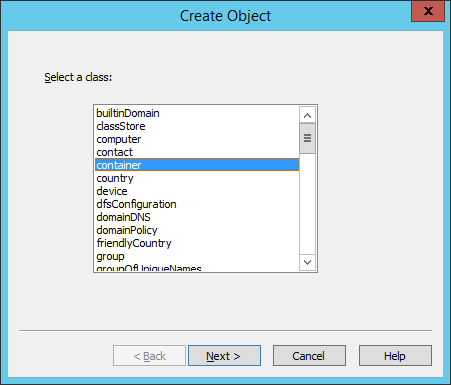
\includegraphics{Screenshots/vmmtest_AD_4.png}
 \captionof{figure}{Creation of the container.}
\end{minipage}
$\;$ \\ \\
\noindent\begin{minipage}{\textwidth}
    \centering
    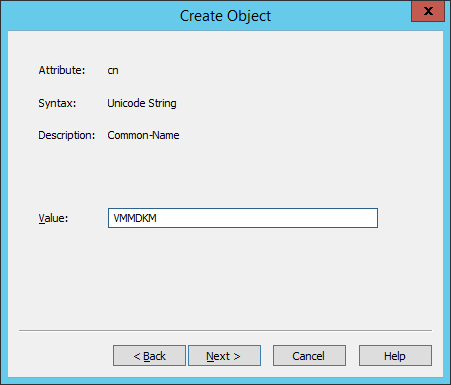
\includegraphics{Screenshots/vmmtest_AD_5.png}
 \captionof{figure}{Creation of the container.}
\end{minipage}
$\;$ \\ \\
Next, some permissions for the VMMDKM container must be set. To do so, right click on the newly created container and select \texttt{Properties}. On the \texttt{Security} tab, click advanced. Click \texttt{Edit}. \\
Make sure the principal is ``VMMService''. and change \texttt{Applies to:} to ``This object and all descendant objects''.
$\;$ \\ \\
\noindent\begin{minipage}{\textwidth}
    \centering
    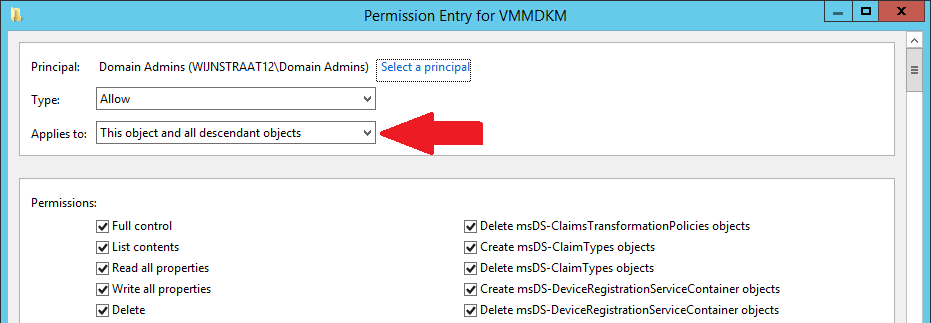
\includegraphics[width=\textwidth]{Screenshots/vmmtest_AD_6.png}
 \captionof{figure}{Configuration of the permissions for VMMDKM.}
\end{minipage}
%$\;$ \\ \\
%\noindent\begin{minipage}{\textwidth}
%    \centering
%    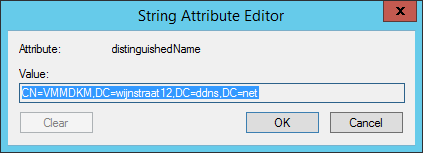
\includegraphics[width=\textwidth]{Screenshots/vmmtest_AD_7.png}
% \captionof{figure}{.}
%\end{minipage}
$\;$ \\ \\
After this, the VMMService account needs to be added to the \textbf{local} administrators group. To do so, open computer management and select \texttt{Local Users and Groups $\rightarrow$ Groups}. Right click on the \texttt{Administrators} group and choose \texttt{Properties} and add the ``VMMService'' account to the group. Click \texttt{OK}.
$\;$ \\ \\
\noindent\begin{minipage}{\textwidth}
    \centering
    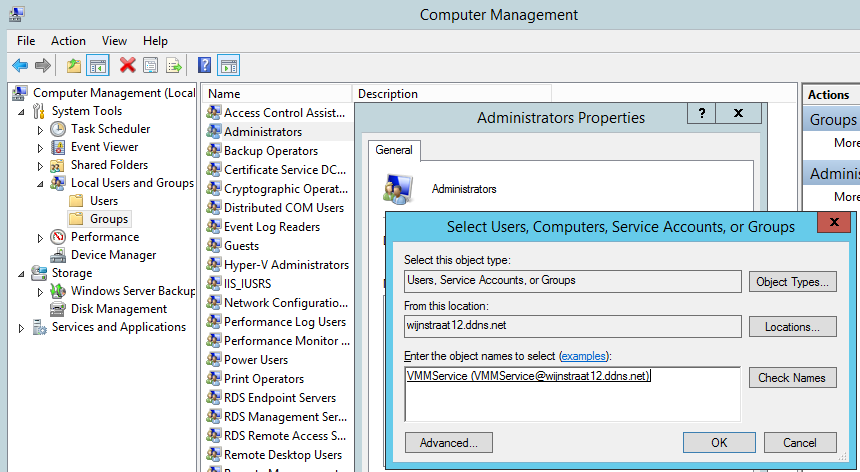
\includegraphics[width=\textwidth]{Screenshots/vmmtest_AD_9.png}
 \captionof{figure}{Adding the VMMService account to the local administrators group.}
\end{minipage}
$\;$ \\

\subsection{Post configuration of MSSQL Server}

The VMMService account has to be given database acccess. Therefore, open ``SQL Server Management Studio'', login using Windows Authentication and expand the \texttt{Security} folder. Right click on \texttt{Logins} and create a new login. This login account is the VMMService account.
$\;$ \\ \\
\noindent\begin{minipage}{\textwidth}
    \centering
    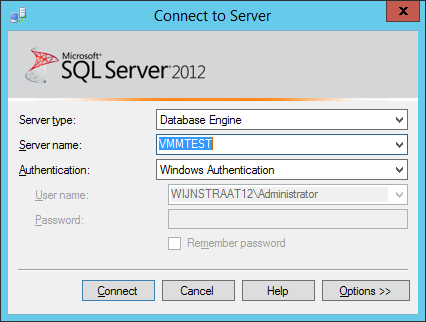
\includegraphics{Screenshots/vmmtest_SQL_9.png}
 \captionof{figure}{Login into SQL Server Management Studio using Windows Authentication.}
\end{minipage}
$\;$ \\ \\
\noindent\begin{minipage}{\textwidth}
    \centering
    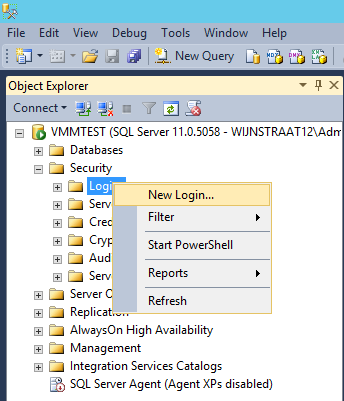
\includegraphics{Screenshots/vmmtest_SQL_10.png}
 \captionof{figure}{Creation of a new login.}
\end{minipage}
$\;$ \\ \\
On the \texttt{Server role} page of this new login, make sure to check the ``dbcreator'', ``process admin'', ``public'' and ``security admin'' roles. After this is completed, exit Management Studio. 
$\;$ \\ \\
\noindent\begin{minipage}{\textwidth}
    \centering
    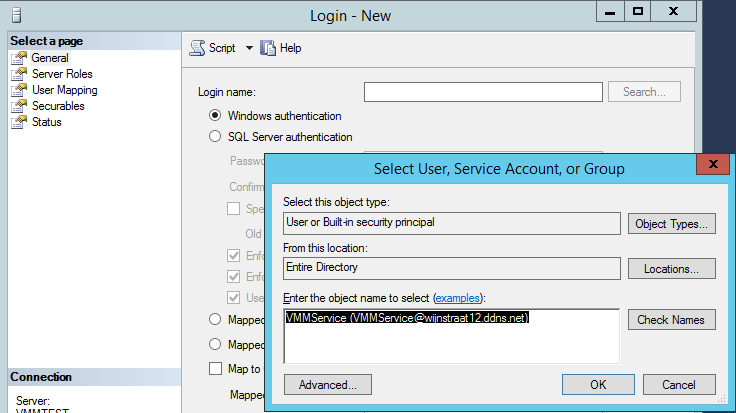
\includegraphics[width=\textwidth]{Screenshots/vmmtest_SQL_11.png}
 \captionof{figure}{Selecting the VMMService account.}
\end{minipage}
$\;$ \\ \\
\noindent\begin{minipage}{\textwidth}
    \centering
    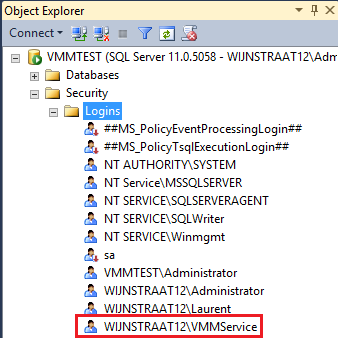
\includegraphics{Screenshots/vmmtest_SQL_12.png}
 \captionof{figure}{Confirmation.}
\end{minipage}
$\;$ \\

\subsection{Installation of VMM}

There is one prerequisite that is not fulfilled yet: the installation of the Windows Assessment and Deployment Kit. Since Windows Server 2012 R2 is used, Windows ADK for Windows 8.1 must be installed. The Windows ADK can be downloaded from the Microsoft website: \url{https://www.microsoft.com/en-us/download/details.aspx?id=39982}
$\;$ \\ \\
\noindent\begin{minipage}{\textwidth}
    \centering
    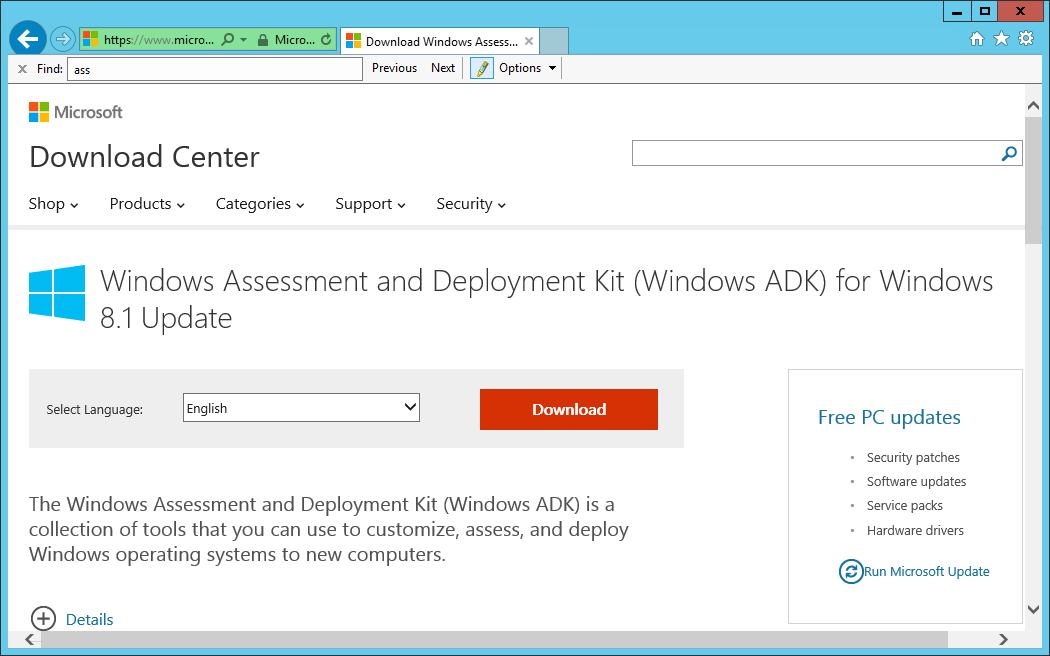
\includegraphics[width=\textwidth]{Screenshots/vmmtest_IE_1.png}
 \captionof{figure}{Download the Windows ADK for Windows 8.1.}
\end{minipage}
$\;$ \\ \\
Since we are installing VMM on the computer we are currently logged into, choose the option ``Install the Windows Assessment and Deployment Kit for Windows 8.1 to this computer''.
$\;$ \\ \\
\noindent\begin{minipage}{\textwidth}
    \centering
    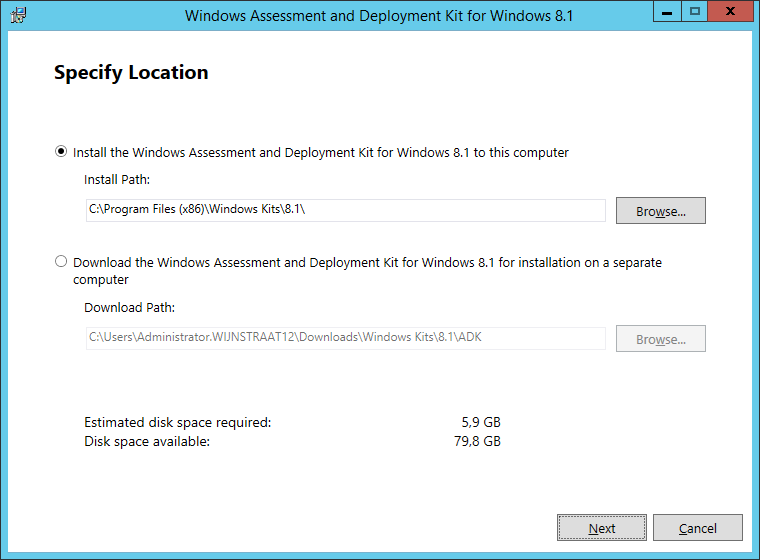
\includegraphics[width=\textwidth]{Screenshots/vmmtest_WADK_1.png}
 \captionof{figure}{Install the ADK on the current compute, since VMM will also be installed on this local computer.}
\end{minipage}
$\;$ \\ \\
Choose whether or not you want to participate with the Customer Experience Improvement Program and acccept the License Agreement. \\
On the ``Select features screen'', make sure you only select ``Deployment Tools'' and ``Windows Preinstallation Environment''. 
$\;$ \\ \\
\noindent\begin{minipage}{\textwidth}
    \centering
    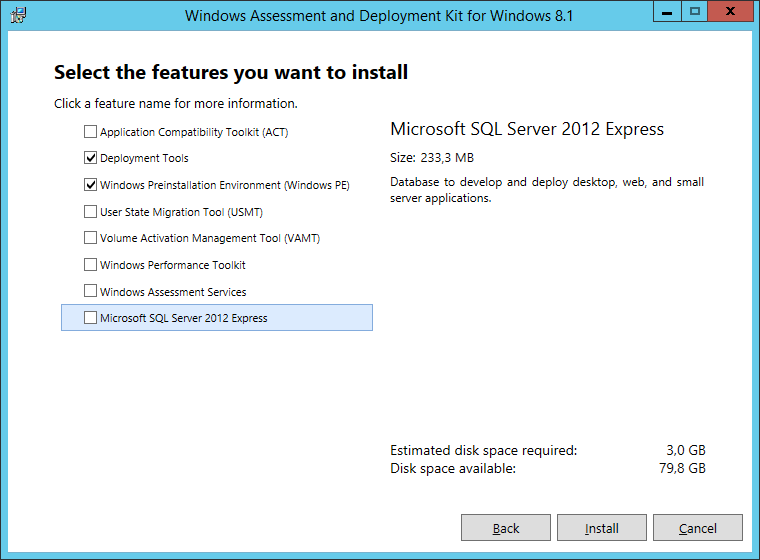
\includegraphics[width=\textwidth]{Screenshots/vmmtest_WADK_2.png}
 \captionof{figure}{Install only the Deployment Tools and Windows PE.}
\end{minipage}
$\;$ \\ \\
Now the actual installation of SCVMM can be started. To do so, double click on the .msi file that has been downloaded from the Microsoft site. After extracting the files, open the folder and double click on \texttt{setup.exe}. The main screen of SCVMM is shown.
$\;$ \\ \\
\noindent\begin{minipage}{\textwidth}
    \centering
    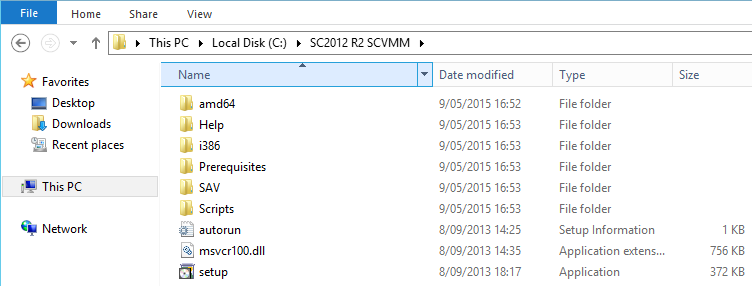
\includegraphics[width=\textwidth]{Screenshots/vmmtest_VMM_1.png}
 \captionof{figure}{Extract the files and double click on \texttt{setup.exe}.}
\end{minipage}
$\;$ \\ \\
Since we want to install VMM, choose for \texttt{Install}.
$\;$ \\ \\
\noindent\begin{minipage}{\textwidth}
    \centering
    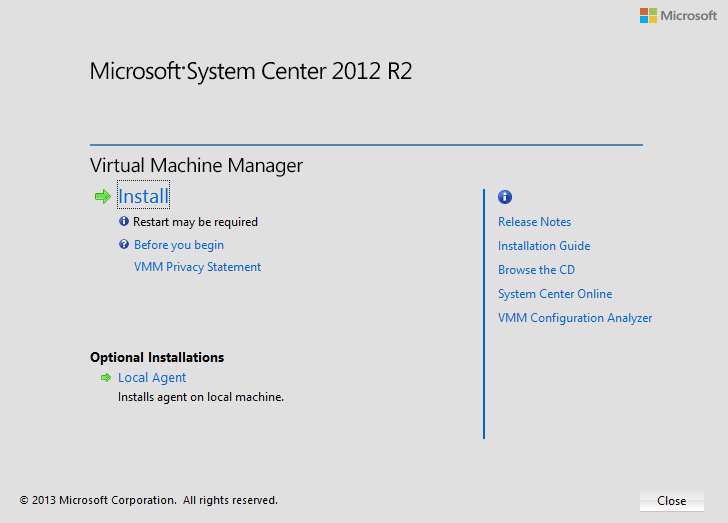
\includegraphics[width=\textwidth]{Screenshots/vmmtest_VMM_2.png}
 \captionof{figure}{The main screen of Virtual Machine Manager 2012 R2 is shown.}
\end{minipage}
$\;$ \\ \\
Select \texttt{VMM management server}, the \texttt{VMM console} is automatically selected as well. The console is the Graphical User Interface of Virtual Machine Manager that allows one to connect to the VMM management server.
$\;$ \\ \\
\noindent\begin{minipage}{\textwidth}
    \centering
    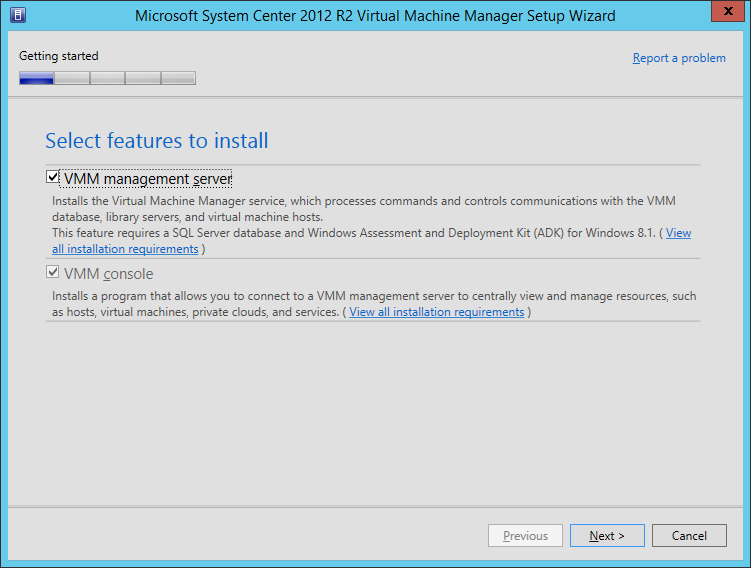
\includegraphics[width=\textwidth]{Screenshots/vmmtest_VMM_3.png}
 \captionof{figure}{Select the VMM management server.}
\end{minipage}
$\;$ \\ \\
Next, the installation location has to be chosen.
$\;$ \\ \\
\noindent\begin{minipage}{\textwidth}
    \centering
    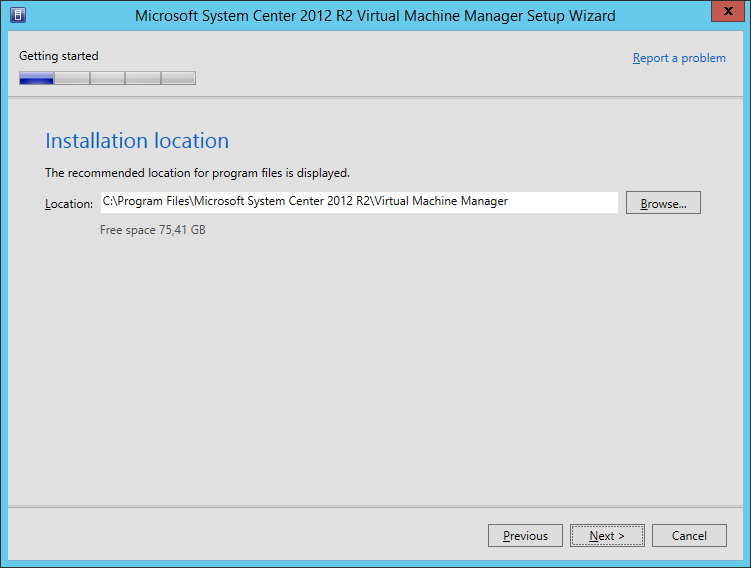
\includegraphics[width=\textwidth]{Screenshots/vmmtest_VMM_4.png}
 \captionof{figure}{Choose the installation location.}
\end{minipage}

\clearpage

On the next screen, the information regarding the database connection and configuration has to be provided. On the \texttt{Server name} field, ``VMMTEST'' or ``localhost'' are both valid names. Leave the \texttt{Port} field empty. The default port is used. \\
We want to login using the VMMService account. This is why we created the login in the previous section. Enter its name and password. Make sure to also provide the NETBIOS domain name of the account in capital letters, followed by a backslash ($\backslash$) before the account name. An example could be: \texttt{WIJNSTRAAT12$\backslash$VMMService}.\\
Specify the \texttt{Instance name} (``MSSQLSERVER'' by default) and select \texttt{New database}.
$\;$ \\ \\
\noindent\begin{minipage}{\textwidth}
    \centering
    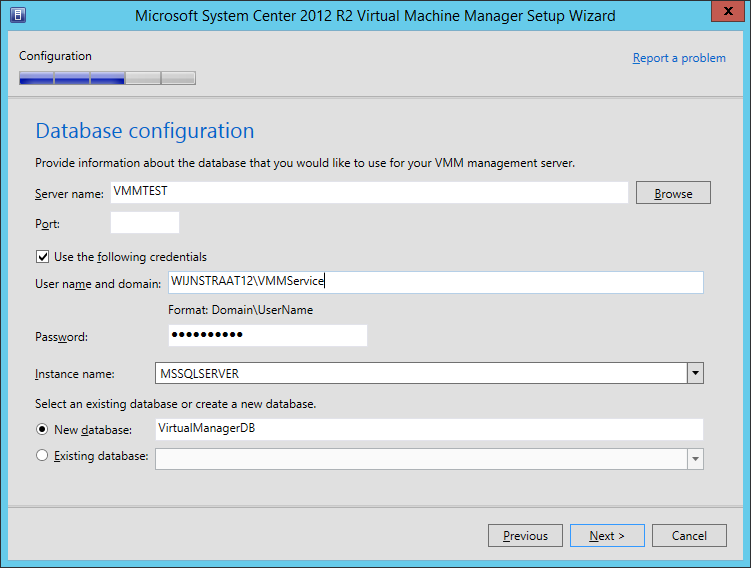
\includegraphics[width=\textwidth]{Screenshots/vmmtest_VMM_5.png}
 \captionof{figure}{Configuration of the database.}
\end{minipage}

\clearpage

Now, Distributed Key Management has to be configured. Another reason why a service account has been configured in the Active Directory. Note that DKM is optional, but if we want to configure a high availability VMM cluster in the future, the prerequisite work is already performed. \\
Provide the same VMMService account as used in the previous step(s). Don't forget to also specify the NETBIOS domain name. \\
Check \texttt{Store my keys in Active Directory} and specify the DN (Distinguished Name) of the VMMDKM container created earlier.
$\;$ \\ \\
\noindent\begin{minipage}{\textwidth}
    \centering
    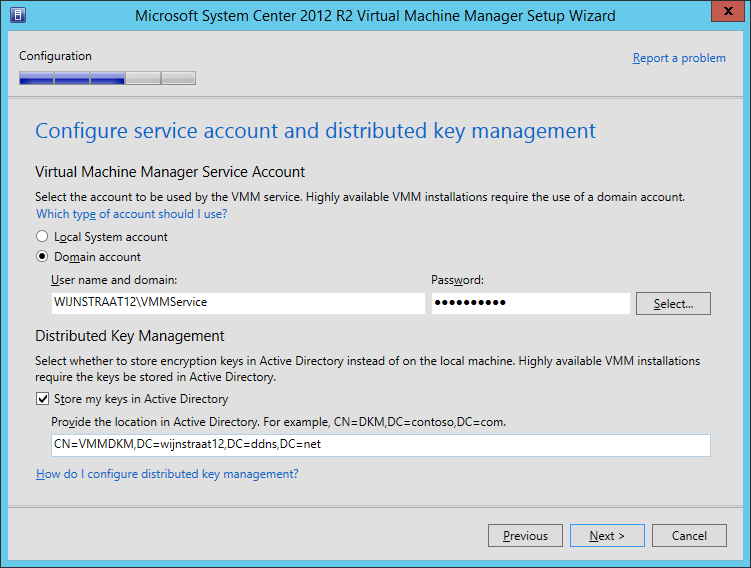
\includegraphics[width=\textwidth]{Screenshots/vmmtest_VMM_6.png}
 \captionof{figure}{.}
\end{minipage}

\clearpage

In the shared library, all your shared files such as .ISO images will be stored. Therefore, it might be a good idea to specify another destination of with more space than the default location. In this example, the default location is used.
$\;$ \\ \\
\noindent\begin{minipage}{\textwidth}
    \centering
    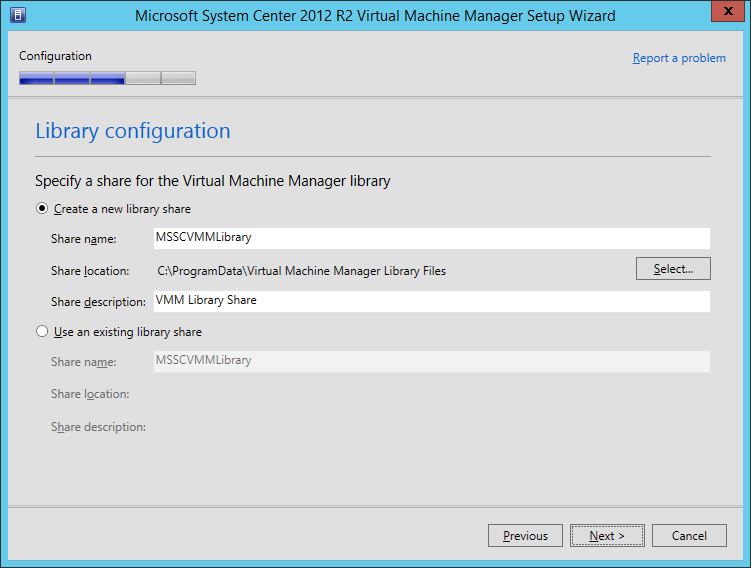
\includegraphics[width=\textwidth]{Screenshots/vmmtest_VMM_7.png}
 \captionof{figure}{Specify the location of the shared libraries.}
\end{minipage}
$\;$ \\ \\
\noindent\begin{minipage}{\textwidth}
    \centering
    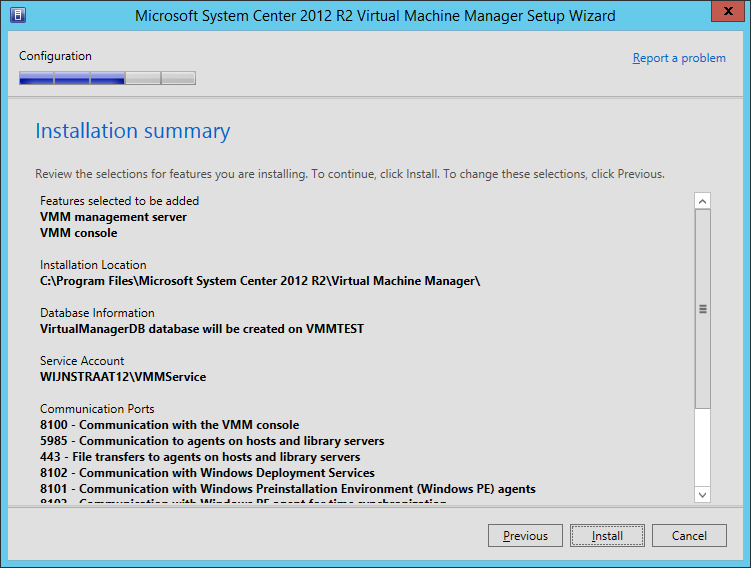
\includegraphics[width=\textwidth]{Screenshots/vmmtest_VMM_8.png}
 \captionof{figure}{Overview of the configuration settings. Click \texttt{Install}.}
\end{minipage}

\section{Installation of Windows Azure Pack}

Windows Azure Pack (formerly known as Windows Azure Services for Windows Server \citep{WAP1}), is a collection of Windows Azure technologies that allows one to build its own private cloud and runs on top of SC Virtual Machine Manager 2012 R2 which, in his turn, runs on top of Windows Server 2012 R2. It basically brings Windows Azure to one's own datacenter \citep{WAP2, WAP3}. \\
Prior to installing Windows Azure Pack, the Service Profider Foundation (SPF) needs to be installed. It offers Infrastructure as a Service (IaaS) and is installed on top of VMM. So basically, the layered infrastructure is like this: \texttt{Windows Server 2012 R2 $\rightarrow$ Virtual Machine Manager 2012 R2  $\rightarrow$ Service Provider Foundation  $\rightarrow$  Windows Azure Pack}. \\ \\
Windows Aure Pack is installed on a dedicated machine called \texttt{windowsazure}. Windows Aure Pack (or WAP for short) requires Microsoft SQL Server 2012 or higher. The SQL Server installed on the VMM virtual machine can be used, or a new, local, instance can be created.

\subsection{Prerequisites}

The installation of Windows Service Provider Foundation requires some additional steps to be performed prior to its installation. The following requirements must be met:
\begin{itemize}
\item Operating System: Windows Server 2012 or higher with PowerShell 3.0.
\item System Center Virtual Machine Manager console SP1 or higher.
\item Web Server IIS Server role with Scripts and Tools, Basic Security, Windows Authentication and ASP.NET 4.5.
\item .NET Framework 4.5 or higher + HTTP Activation.
\item Management OData IIS Extension.
\item WCF Data Services 5.0 for OData V3.
\item ASP.NET MVC 4
\end{itemize}
The installation of all the prerequisites will be covered in this manual. As previously said, WAP is installed on a dedicated VM with a fresh install of Windows Server 2012 R2. The server is given a static IP address and is made member of the same AD domain that the VMM server is running in. That is, \texttt{wijnstraat12.ddns.net}.
$\;$ \\ \\
\noindent\begin{minipage}{\textwidth}
    \centering
    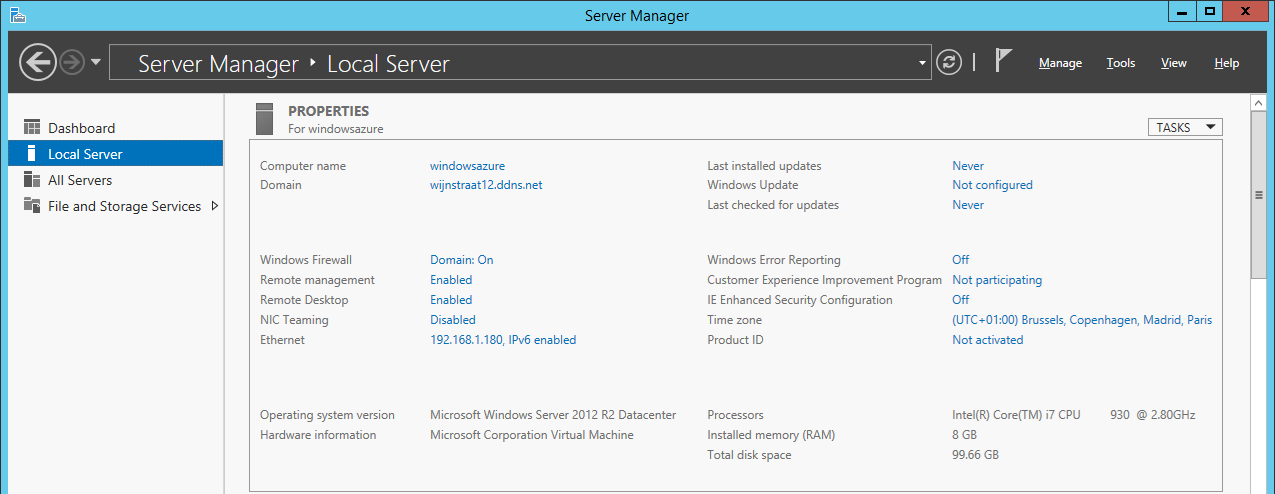
\includegraphics[width=1\textwidth]{Screenshots/WAP_1.png}
 \captionof{figure}{Overview screen of the local server showing the begin situation.}
\end{minipage}
When choosing an installation of a new instance of SQL Server, make sure to select \texttt{Mixed Mode} as authentication mode. When reusing the existant instance of SQL Server, additional configuration will have to be performed in order to be able to install the WAP.
$\;$ \\ \\
\noindent\begin{minipage}{\textwidth}
    \centering
    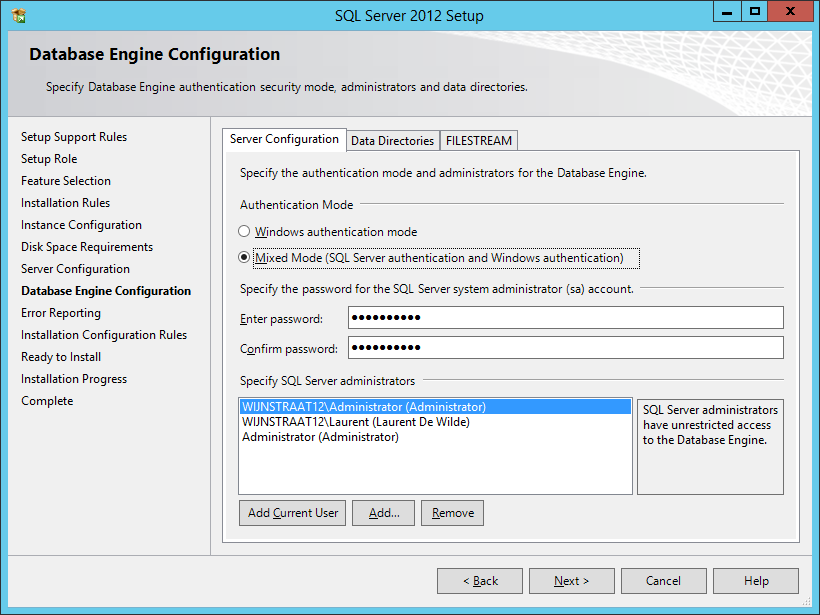
\includegraphics[width=\textwidth]{Screenshots/WAP_2.png}
 \captionof{figure}{Authentication Mode: Mixed Mode.}
\end{minipage}

\clearpage

Now the server is ready to install the prerequisites. The installation of the VMM console is the first requirement and can be installed from the VMM installation media. \\
Extract the files of the .msi file and lauch \texttt{setup.exe}. Choose \texttt{Install} and check \texttt{VMM console}. Click \texttt{Install} on the confirmation screen.
$\;$ \\ \\
\noindent\begin{minipage}{\textwidth}
    \centering
    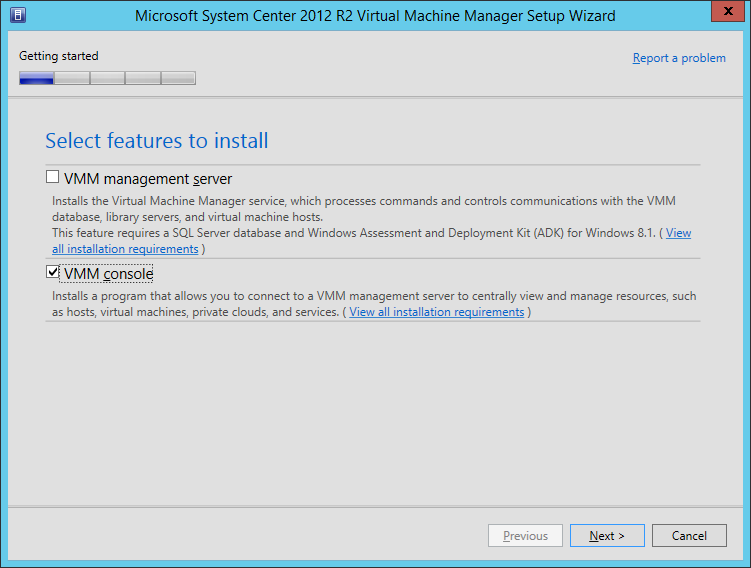
\includegraphics[width=\textwidth]{Screenshots/WAP_3.png}
 \captionof{figure}{Install only the VMM console.}
\end{minipage}

\clearpage

Next step is the installation of the Web Server (IIS). Therefore, open \texttt{Add roles and services} from the Server Manager and check \texttt{Web Server (IIS)}. Click \texttt{Next}.
$\;$ \\ \\
\noindent\begin{minipage}{\textwidth}
    \centering
    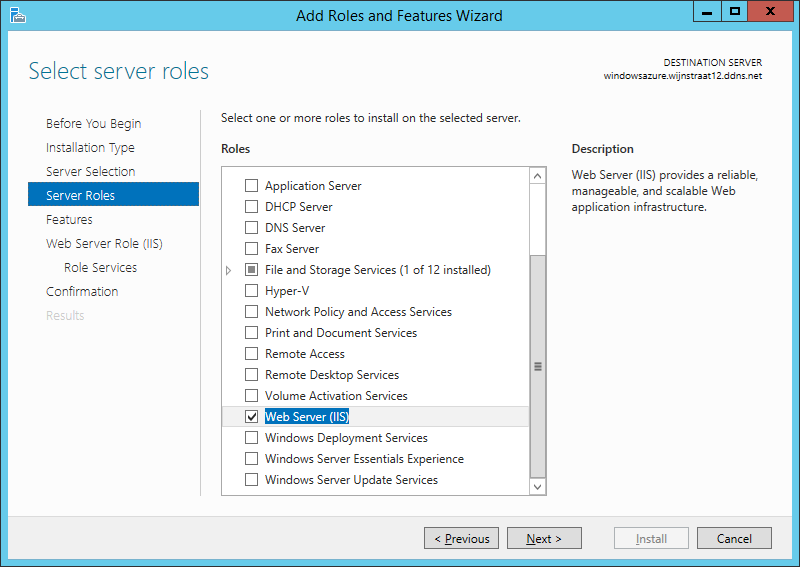
\includegraphics[width=\textwidth]{Screenshots/WAP_5.png}
 \captionof{figure}{Select the \texttt{Web Server (IIS)} Server Role.}
\end{minipage}

\clearpage

On the \texttt{Features} screen, select the following features:
\begin{itemize}
\item \texttt{.NET Framework 4.5 Features $\rightarrow$ WCP Services $\rightarrow$ HTTP Activation}
\item \texttt{Management OData IIS Extension} and its associated features.
\end{itemize}
$\;$ \\ \\
\noindent\begin{minipage}{\textwidth}
    \centering
    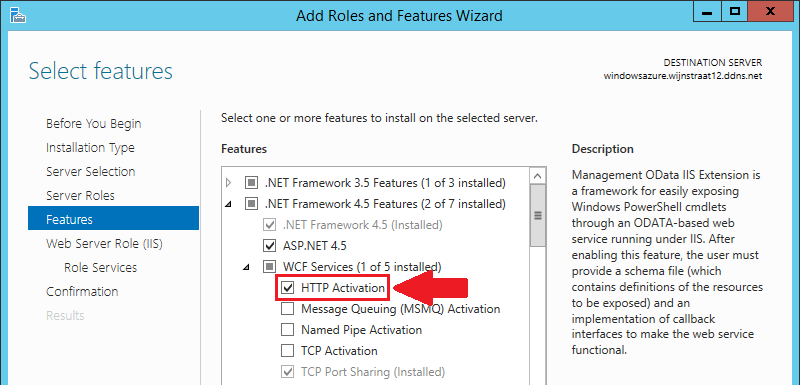
\includegraphics[width=\textwidth]{Screenshots/WAP_6.png}
 \captionof{figure}{Select \texttt{HTTP Activation}.}
\end{minipage}
$\;$ \\ \\
\noindent\begin{minipage}{\textwidth}
    \centering
    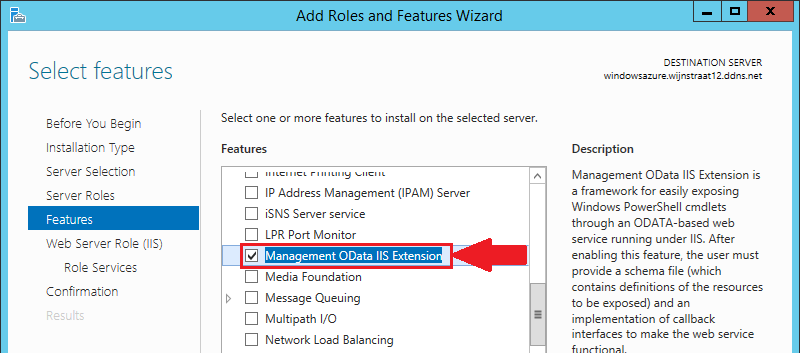
\includegraphics[width=\textwidth]{Screenshots/WAP_7.png}
 \captionof{figure}{Select \texttt{Management OData IIS Extension}.}
\end{minipage}

\clearpage

On the \texttt{Web Server Role (IIS) - Role Services} screen, select following role services:
\begin{itemize}
\item \texttt{IIS Management $\rightarrow$ Scripts and Tools}
\item \texttt{Security $\rightarrow$ Basic Authentication}
\item \texttt{Security $\rightarrow$ Windows Authentication}
\item \texttt{Application Development $\rightarrow$ .NET 4.5}
\end{itemize}
$\;$ \\ \\
\noindent\begin{minipage}{\textwidth}
    \centering
    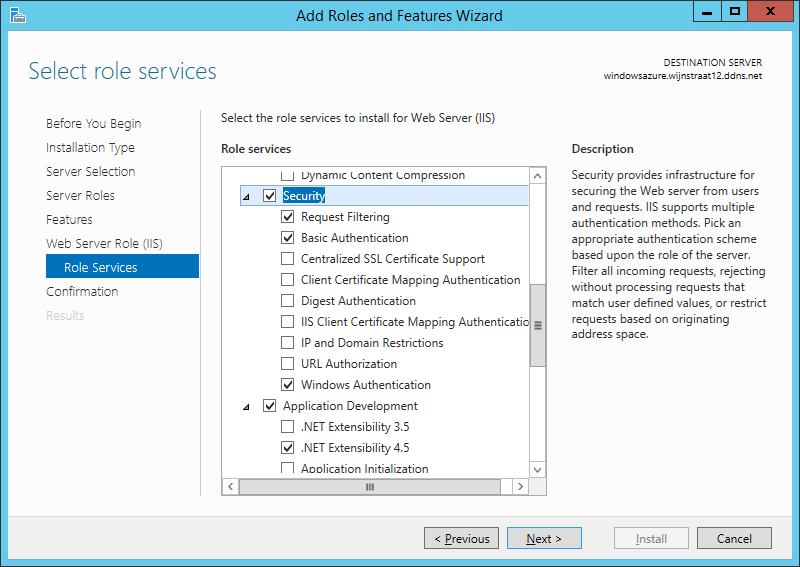
\includegraphics[width=\textwidth]{Screenshots/WAP_8.png}
 \captionof{figure}{.}
\end{minipage}

\clearpage

Some additional software needs to be installed being \texttt{WCF Data Services 5.0 for OData V3} and \texttt{ASP.NET MVC 4}. \\
The \texttt{WCF Data Services 5.0 for OData V3} can be downloaded from this location: \url{https://www.microsoft.com/en-us/download/details.aspx?id=29306}. The installtion is straightforward and will not be covered. Just execute the installer, accept the License Agreement and  click \texttt{Install}.\\
\texttt{ASP.NET MVC 4} can be download from the following location: \url{https://www.microsoft.com/en-us/download/details.aspx?id=30683}. The installation is roughly the same as the WCF Data Services.
$\;$ \\ \\
\noindent\begin{minipage}{\textwidth}
    \centering
    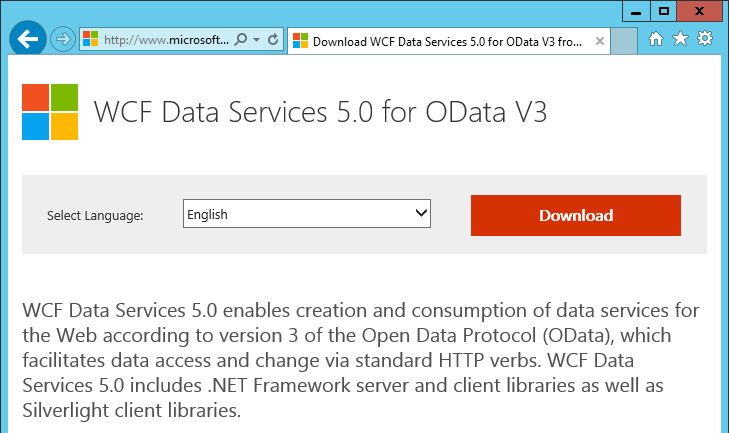
\includegraphics[width=0.7\textwidth]{Screenshots/WAP_9.png}
 \captionof{figure}{Download and install WCF Data Services for OData V3.}
\end{minipage}
$\;$ \\ \\
\noindent\begin{minipage}{\textwidth}
    \centering
    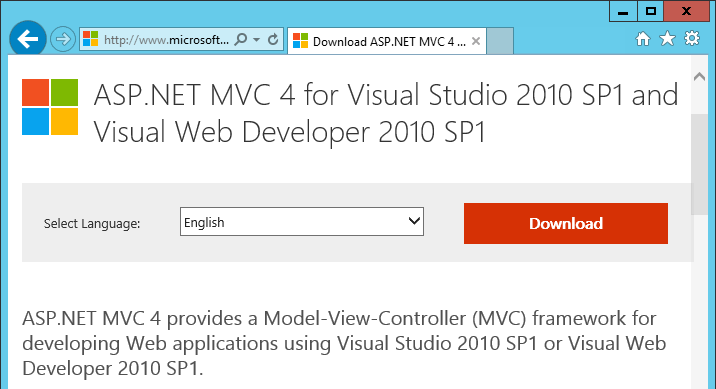
\includegraphics[width=0.7\textwidth]{Screenshots/WAP_11.png}
 \captionof{figure}{Download and install ASP.NET MVC 4.}
\end{minipage}
$\;$ \\ \\
Also for the Service Provider Foundation, a service accounts needs to be made. Therefore, add a domain user in the Active Directory called \texttt{SPFService}. Make sure the password never expires. \\
Four additional domain groups need to be made for setting permissions on the directories created by the installer. Those four groups are: \texttt{SPFAdmins}, \texttt{SPFProvider}, \texttt{SPFUsage} and \texttt{SPFVMM}.
$\;$ \\ \\
\noindent\begin{minipage}{\textwidth}
    \centering
    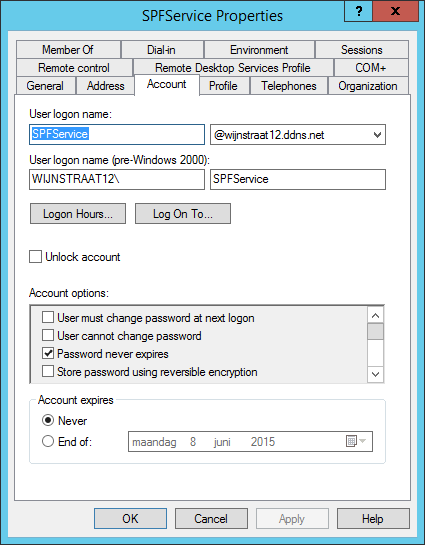
\includegraphics{Screenshots/WAP_13.png}
 \captionof{figure}{The properties of the domain account \texttt{SPFService}.}
\end{minipage}
$\;$ \\ \\
\noindent\begin{minipage}{\textwidth}
    \centering
    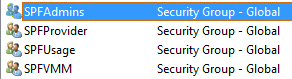
\includegraphics{Screenshots/WAP_14.png}
 \captionof{figure}{The four global security groups have been made.}
\end{minipage}
$\;$ \\ \\
Communications to and from the webserver should be secured / encrypted by SSL, which requires certificates. Two types of certificates exist: self-signed certificates and certificartes issued by a standalone certification authority.  \\
In our case, the Windows Azure Pack will be installed on the same domain as the Service Provider Foundation and thus we are not required to use a public certificate issued by a standalone certification authority. So self-singed certificates will be used. \\
Installing such a certificate is done by using IIS Manager. Open it and select the webserver in the \texttt{Connections} pane. Next, click \texttt{Server Certificates} in the main window. On the \texttt{Actions} pane, click \texttt{Create Self-Singed Certificate}. \\
Specify the common name. Keep in mind that the common name must match the URL that is used when connecting to the Service Provider Foundation.
$\;$ \\ \\
\noindent\begin{minipage}{\textwidth}
    \centering
    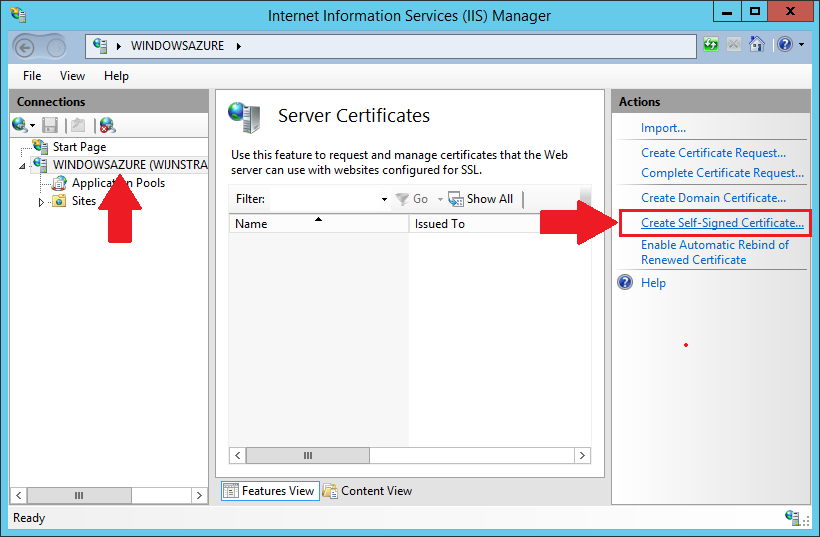
\includegraphics[width=0.9\textwidth]{Screenshots/WAP_15.png}
 \captionof{figure}{Create a self-singed certificate.}
\end{minipage}
$\;$ \\ \\
Now the installation of Service Provider Foundation can be started. The SPF can be found as a standalone installation on the System Center Orchestrator installation media. Extract the files of System Center Orchestrator, double click on \texttt{setup.exe} and select \texttt{Service Provider Foundation}.
$\;$ \\ \\
\noindent\begin{minipage}{\textwidth}
    \centering
    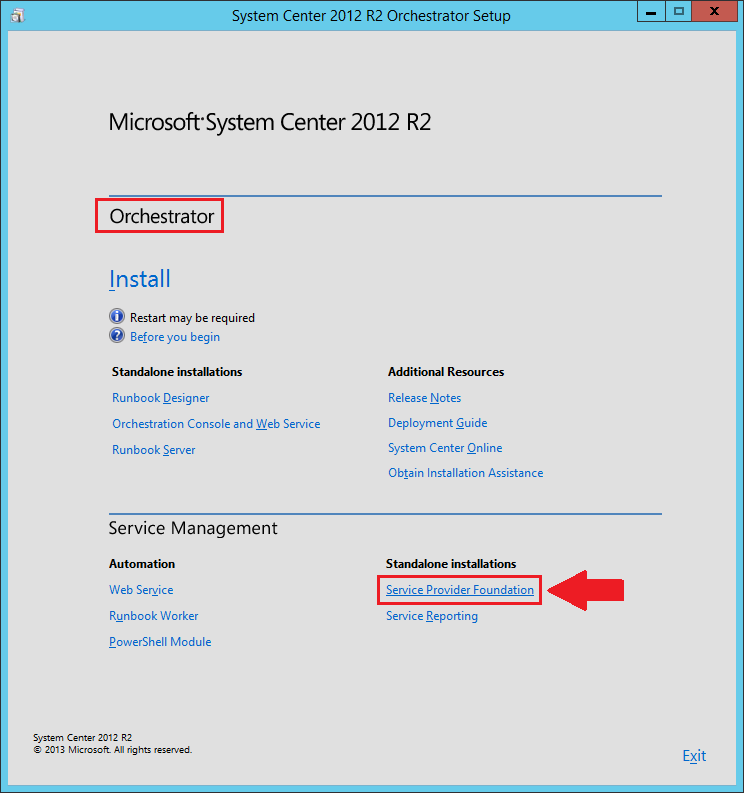
\includegraphics[width=\textwidth]{Screenshots/WAP_16.png}
 \captionof{figure}{SPF can be found on the SC Orchestrator installation media.}
\end{minipage}
$\;$ \\ \\
The installer will check if al the prerequisites have been met.
$\;$ \\ \\
\noindent\begin{minipage}{\textwidth}
    \centering
    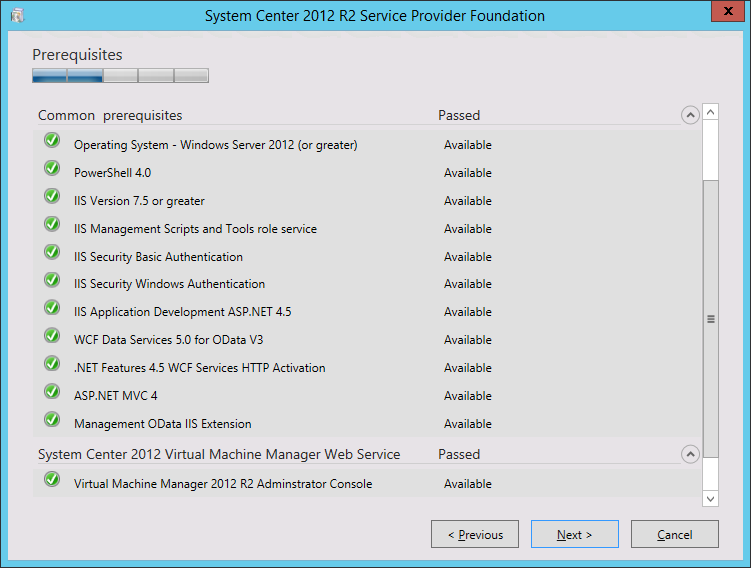
\includegraphics[width=\textwidth]{Screenshots/WAP_17.png}
 \captionof{figure}{The prerequisites are checked. When everything is installed, setup can be continued.}
\end{minipage}
$\;$ \\ \\
Next, the database server location where the SPF database will be created, has to be configured. Either use the newly created, local SQL instance or use the SQL Server created earlier when setting up the VMM. In both cases, make sure the firewall allows both incoming and outgoing traffic on port 1433.
$\;$ \\ \\
\noindent\begin{minipage}{\textwidth}
    \centering
    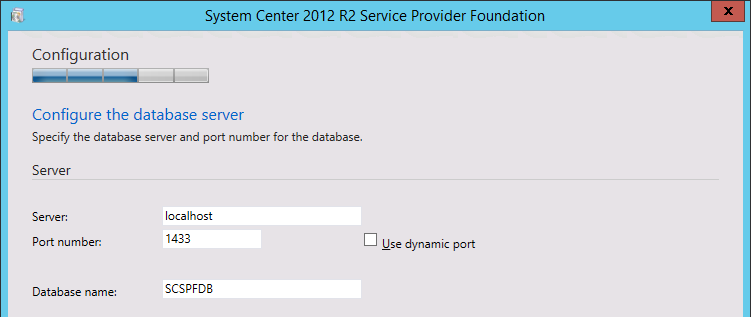
\includegraphics[width=\textwidth]{Screenshots/WAP_18.png}
 \captionof{figure}{Configuration of the database. A newly created instance can be used, as well as the instance created earlier when setting up the VMM virtual machine.}
\end{minipage}
$\;$ \\ \\
Then the certificate for the web service has to be selected. Since we already created a certificate, select \texttt{Use existing certificate:} and select the correct certificate.
$\;$ \\ \\
\noindent\begin{minipage}{\textwidth}
    \centering
    \includegraphics[width=\textwidth]{Screenshots/WAP_19.png}
 \captionof{figure}{Certificate selection. Choose the self-singed certificate created earlier.}
\end{minipage}

\clearpage

Now, the configuration of the virtual directories of IIS, permissions and App Pool Identities have to be configured. In the next four steps, the four domain groups created earlier need to be specified in each step. The service account \texttt{SPFService} is used in all steps.
$\;$ \\ \\
\noindent\begin{minipage}{\textwidth}
    \centering
    \includegraphics[width=\textwidth]{Screenshots/WAP_20.png}
 \captionof{figure}{Configuration of the \texttt{Admin} virtual directory of IIS. Choose the \texttt{SPFAdmin} and the \texttt{SPFService} service account, both created earlier in the pre-setup process.}
\end{minipage}
$\;$ \\ \\
\noindent\begin{minipage}{\textwidth}
    \centering
    \includegraphics[width=\textwidth]{Screenshots/WAP_21.png}
 \captionof{figure}{Configuration of the \texttt{Provider} virtual directory of IIS. Choose the \texttt{SPFProvider} and the \texttt{SPFService} service account, both created earlier in the pre-setup process.}
\end{minipage}
$\;$ \\ \\
Then the VMM web service and the Usage web service have to be specified. Use \texttt{SPFVMM} and \texttt{SPFUsage} respectively for this purposes. The service account remains the same: \texttt{SPFService}.

\clearpage

\subsection{Post Installation of Service Provider Foundation}

In order to use Windows Azure Pack correctly, some additional configuration must be performed. The \texttt{SPFService} account must be given additional permissions. It needs to be added as a member of the following \textbf{local} groups:
\begin{itemize}
\item SPF\_Admin
\item SPF\_Provider
\item SPF\_Usage
\item SPF\_VMM
\end{itemize}
Double click on either one of them, click \texttt{Add\ldots} and search for the \texttt{SPFService} account. Click \texttt{OK}. Repeat this process for the other groups.
$\;$ \\ \\
\noindent\begin{minipage}{\textwidth}
    \centering
    \includegraphics[width=\textwidth]{Screenshots/WAP_22.png}
 \captionof{figure}{Add the \texttt{SPFService} account to the local groups created by the Service Provider Foundation installation.}
\end{minipage}

\clearpage

The \texttt{SPFService} account also needs to be added to the Administrator user role in VMM. To do so, open VMM (either the console installed on this VM or on the VMM virtual machine itself). Click on \texttt{Settings} in the bottom-left corner and click on \texttt{Security $\rightarrow$ User Roles}. Double click on the \texttt{Administrator} user role and on the \texttt{Members} tab, click \texttt{Add\ldots} to add the \texttt{SPFService} account to the user role.
$\;$ \\ \\
\noindent\begin{minipage}{\textwidth}
    \centering
    \includegraphics[width=\textwidth]{Screenshots/WAP_23.png}
 \captionof{figure}{The \texttt{SPFService} account needs administrative permissions in Virtual Machine Manager.}
\end{minipage}

\clearpage

The \texttt{SPFService} account needs permissions in the SQL Server as well. To set those permissions, open SQL Server Management Studio and navigate to \texttt{Security $\rightarrow$ Logins} and double click on \texttt{WIJNSTRAAT12$\backslash$SPFService}. Select the \texttt{Server Roles} tab and check \texttt{sysadmin}.
$\;$ \\ \\
\noindent\begin{minipage}{\textwidth}
    \centering
    \includegraphics[width=\textwidth]{Screenshots/WAP_24.png}
 \captionof{figure}{Adding administrative permissions to the \texttt{SPFService} account.}
\end{minipage}
$\;$ \\ \\
To verify the correct Application Pool settings of the web service, make sure that the identity of the Application Pools \texttt{Admin}, \texttt{Provider}, \texttt{Usage} and \texttt{VMM} is set to \texttt{WIJNSTRAAT12$\backslash$SPFService}. \\
To do so, open IIS Manager and select the \texttt{WINDOWSAZURE} web server. In the \texttt{Actions} pane on the right, click on \texttt{View Application Pools}.
$\;$ \\ \\
\noindent\begin{minipage}{\textwidth}
    \centering
    \includegraphics[width=\textwidth]{Screenshots/WAP_25.png}
 \captionof{figure}{Verifying the correct settings of the Application Pools.}
\end{minipage}
$\;$ \\ \\
To register the Service Provider Foundation in Windows Azure Pack, a \textbf{local} account has to be made on the same computer on where WAP will be installed. In our case, this is the current virtual machine we are working on. \\
Therefore, create a \textbf{local} user account named \texttt{SPF\_REG} and make it a member of the following groups:
\begin{itemize}
\item SPF\_Admin
\item SPF\_Provider
\item SPF\_VMM
\item SPF\_Usage
\end{itemize}
$\;$ \\
\noindent\begin{minipage}{\textwidth}
    \centering
    \includegraphics[width=0.5\textwidth]{Screenshots/WAP_26.png}
 \captionof{figure}{Creation of the local \texttt{SPF\_REG} account.}
\end{minipage}
$\;$ \\ \\
\noindent\begin{minipage}{\textwidth}
    \centering
    \includegraphics[width=0.5\textwidth]{Screenshots/WAP_27.png}
 \captionof{figure}{The account has been added to the four local groups created by the SPF installer.}
\end{minipage}

\clearpage

\subsection{Installation of the Windows Azure Pack}

Two possibilities exist to install WAP: single server installation or distributed installation. The single server installation has been chosen, so this manual will focus on the installation of all the components of WAP on one server. \\
To install the Windows Azure Pack on a single server, download and run the Web Platform Installer 5.0, which can be downloaded from the Microsoft website: \url{http://www.microsoft.com/web/downloads/platform.aspx}. \\
On the \texttt{Products} tab, on the left pane select \texttt{Windows Azure} and add \texttt{Windows Azure Pack: Portal and API Express} with all its dependencies. Click \texttt{Next}.
$\;$ \\ \\
\noindent\begin{minipage}{\textwidth}
    \centering
    \includegraphics[width=\textwidth]{Screenshots/WAP_28.png}
 \captionof{figure}{Selection of the WAP Portal and API Express.}
\end{minipage}
$\;$ \\ \\
\noindent\begin{minipage}{\textwidth}
    \centering
    \includegraphics[width=\textwidth]{Screenshots/WAP_29.png}
 \captionof{figure}{Click \texttt{Next}.}
\end{minipage}
$\;$ \\ \\
\noindent\begin{minipage}{\textwidth}
    \centering
    \includegraphics[width=\textwidth]{Screenshots/WAP_30.png}
 \captionof{figure}{The installation has completed successfully. Click \texttt{Finish}.}
\end{minipage}

\clearpage
After the installation has finished, go to \url{https://localhost:30101} from where the setup will be continued. \\
The first step is configuring the database connection which WAP will use. Fill in the appropriate server name, for example \texttt{localhost} or the name of the virtual machine that runs VMM and thus also runs an instance of SQL Server. \\
Choose \texttt{SQL Server Authentication} and let the database server admin name be \texttt{sa}. Fill in the password. \\
Then, choose a catchphrase. The use of a catchphrase requires SQL Authentication. When using an existing SQL Server instance using Windows Authentication (for example, the one configured on the VMM), setting up a catchphrase will not work. The security authentication mode needs to be changed to SQL Server and Windows Authentication mode. A guide to do so, can be found here: \url{https://technet.microsoft.com/en-us/library/ms188670.aspx}. \\
When a local instance has been created and Mixed Authentication Mode has been selected during installation, further configuration is not required.
$\;$ \\ \\
\noindent\begin{minipage}{\textwidth}
    \centering
    \includegraphics[width=\textwidth]{Screenshots/WAP_31.png}
 \captionof{figure}{Configuration of the database access for use with WAP.}
\end{minipage}
$\;$ \\ \\
Choose whether or not you want to participate to the Customer Experience Improvement Program and go to the final page (3). \\
The \texttt{Features Setup} page shows which features will be configured. When clicking on the checkmark at the right bottom of the page, the configuration will start. When everything is configured successfully, green checkmarks will appear in before the configuration role as illustrated in the figure below.
$\;$ \\ \\
\noindent\begin{minipage}{\textwidth}
    \centering
    \includegraphics{Screenshots/WAP_32.png}
 \captionof{figure}{Setup has completed successfully.}
\end{minipage}

\clearpage

The installation and configuration of WAP has been completed successfully! Now we have to login into WAP and configure a cloud. \\
Therefore, go to \url{https://localhost:30091} and log in using the \textbf{local} administrator account. To force Windows using the the local account, use a ``\texttt{.$\backslash$}'' before the account name. An example would be: \texttt{.$\backslash$Administrator}.
$\;$ \\ \\
\noindent\begin{minipage}{\textwidth}
    \centering
    \includegraphics[width=\textwidth]{Screenshots/WAP_33.png}
 \captionof{figure}{Login using the local administrator account.}
\end{minipage}
$\;$ \\ \\
\noindent\begin{minipage}{\textwidth}
    \centering
    \includegraphics[width=\textwidth]{Screenshots/WAP_34.png}
 \captionof{figure}{The main screen of WAP.}
\end{minipage}
$\;$ \\ \\
Now, the configuration of a VM cloud can be started. Select \texttt{VM Clouds} in the left pane. First, the Service Provider Foundation Endpoint must be registered using the local account \texttt{SPF\_REG} created earlier. \\
However, in the past I received error messages saying that the registration of the SPF Endpoint could not be completed. The solution is as follows: reset the password of the \texttt{SPF\_REG} account using the \texttt{Local Users and Groups} snap-in. Right click on the \texttt{SPF\_REG} account and choose \texttt{Set password\ldots}. \\
After that, the IIS Web Server needs to be reset. To do so, open PowerShell and execute following command: \texttt{iisreset.exe}.
$\;$ \\ \\
\noindent\begin{minipage}{\textwidth}
    \centering
    \includegraphics[width=\textwidth]{Screenshots/WAP_35.png}
 \captionof{figure}{Before setting up a VM cloud, the SPF Endpoint needs to be registered.}
\end{minipage}
$\;$ \\ \\
\noindent\begin{minipage}{\textwidth}
    \centering
    \includegraphics{Screenshots/WAP_36.png}
 \captionof{figure}{In case of failure, reset the password for the \texttt{SPF\_REG} account.}
\end{minipage}
$\;$ \\ \\
\noindent\begin{minipage}{\textwidth}
    \centering
    \includegraphics{Screenshots/WAP_37.png}
 \captionof{figure}{Restart the Web Server \ldots}
\end{minipage}
$\;$ \\ \\
\noindent\begin{minipage}{\textwidth}
    \centering
    \includegraphics[width=\textwidth]{Screenshots/WAP_38.png}
 \captionof{figure}{\ldots and everything should work fine now.}
\end{minipage}
$\;$ \\ \\
To manage a VM cloud, we must first connect to the VMM server. The existing cloud in VMM will be displayed in the \texttt{VM Clouds}.  \\
Therefore, fill in the Virtual Machine Manager server FQDN: \texttt{vmmtest.wijnstraat12.ddns.net}.
$\;$ \\ \\
\noindent\begin{minipage}{\textwidth}
    \centering
    \includegraphics[width=\textwidth]{Screenshots/WAP_39.png}
 \captionof{figure}{Connect to the VMM server.}
\end{minipage}
$\;$ \\ \\
\noindent\begin{minipage}{\textwidth}
    \centering
    \includegraphics[width=\textwidth]{Screenshots/WAP_40.png}
 \captionof{figure}{The cloud is now visible in \texttt{VM clouds}.}
\end{minipage}

